\title{LEZIONE 10 05/05/2020}\newline
\textbf{link} \href{https://web.microsoftstream.com/video/7c71a45c-bec9-4bd9-b9f1-d200f427542e}{clicca qui}
\section{Bilancio di Potenze (BdP)}
\subsection{Introduzione}
Il principio di D'Alambent non è sempre l'approccio più conveniente per studiare la dinamica di un sistema, esso, infatti, ci consente di determinare pienamente il moto del sistema, ma ci obbliga a calcolare le reazioni vincolari. In molte situazioni può risultare più conveniente usare un \textbf{approccio energetico}.\newline
\newline
Tramite il bilancio di potenze riusciremo a calcolare il moto del sistema senza dover introdurre le reazioni vincolari.\newline
\newline
Il \textbf{bilancio di potenze} si può usare solo in presenza di vincoli:
\begin{itemize}
    \item \textbf{fissi}: senza giochi o cedimenti;
    \item \textbf{perfetti}: non presenta attrito;
    \item \textbf{bilateri}: vale in entrambe le direzioni.
\end{itemize}
\ \newline
Sotto questa ipotesi il bilancio di potenze ci consente di dire: è condizione necessaria e sufficiente per l'\textbf{equilibrio dinamico} di un sistema di corpi rigidi è che si annulli in ogni istante di tempo la potenza delle forze di coppie attive interne ed esterne applicate al sistema, incluse le forze e coppie di inerzia.\newline
\newline
L'\textbf{equazione che regola il bilancio di potenze} è:
\[
    W + W_{in} = 0 \;\;\;\;\;\forall t
\]
con $W$ potenza di forze e coppie attive, $W_{in}$ potenza di coppie e forze di inerzia.\newline
\newline
Definiamo \textbf{potenza di una forza} $\vec{F}$ il termine
\[
    W = \vec{F} \;\text{x}\; \vec{v} [Watt] = F v cos(\theta)
\]
con $\vec{v}$ la velocità del punto di applicazione della forza e $\theta$ l'angolo compreso fra $\vec{F}$ e $\vec{v}$.\newline
\newline
Definiamo \textbf{potenza di una coppia} $\vec{C}$ il termine
\[
    W = \vec{C} \;\text{x}\; \vec{\omega}
\]
con $\vec{\omega}$ la velocità di rotazione del corpo a cui la coppia è applicata.
\newline
\newline
Riscriviamo ora l'equazione che regola il bilancio di potenze:
\[
    \sum_i \vec{F}_i \;\text{x}\; \vec{v}_i + \sum_j \vec{C}_j \;\text{x}\;\vec{\omega}_j + \sum_{i=1}^{n_c}\left( \vec{F}_{in,i} \;\text{x}\;\vec{v}_{G,i} + \vec{C}_{in,i} \;\text{x}\;\vec{\omega}_i \right) = 0
\]
\ \newline
Grazie a questa equazione possiamo:
\begin{itemize}
    \item note le forze e coppie attive applicate al sistema, ottenere lo stato di moto;
    \item noto lo stato di moto, ottenere le forze e coppie attive necessarie per mantenere il moto.
\end{itemize}
Notiamo che nell'equazione non compaiono le reazioni vincolari, questo perchè abbiamo preso come ipotesi dei vincoli ideali.\newline
\newline
Ricordando che $\vec{F}_{in} = - m \vec{a}_{G,i}$ e $\vec{C}_{in} = - J_G \dot{\vec{\omega}}$, allora possiamo riscrivere le potenze delel forze e coppie di inerzia come:
\[
    W_{in} = - \sum_{i=1}^{n_c} \left( m-i \vec{a}_{G,i} \;\text{x}\; \vec{v}_{G,i} + J_{G,i} \dot{\vec{\omega}}_i \;\text{x}\;\vec{\omega}_i \right) = - \frac{d E_c}{dt}
\]
\newline
\subsection{Energia cinetica e teorema di Konig}
Cominciamo definendo l'energia cinetica per un \textbf{punto materiale}:\newline
[immagine dagli appunti del prof]
\begin{center}
    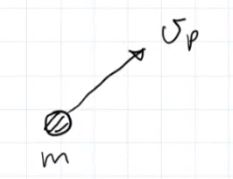
\includegraphics[height=3cm]{../lezione10/img1.JPG}
\end{center}
\[
    E_c = \frac{1}{2} m v_p^2 = \frac{1}{2}m \vec{v}_p \;\text{x}\;\vec{v}_p
\]
\ \newline
Esteniamo ora il concetto a un \textbf{copro rigido}:\newline
[immagine dagli appunti del prof]
\begin{center}
    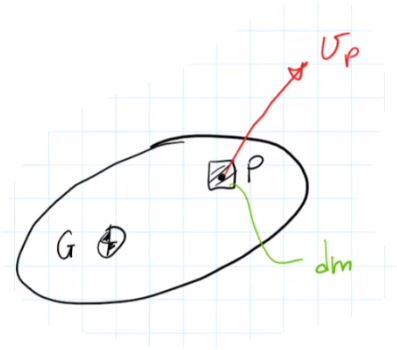
\includegraphics[height=3cm]{../lezione10/img2.JPG}
\end{center}
\[
    dE_c = \frac{1}{2} v_p^2 dm = \frac{1}{2} v_p^2 \rho dV
\]
\[
    E_c = \frac{1}{2} \int_V v_p^2 \rho dV = \frac{1}{2} \int_V \vec{v}_p \;\text{x}\; \vec{v}_p \rho dV
\]
e usando Rivals: $\vec{v}_p = \vec{v}_G + \vec{\omega} \land (P-G)$
\[
    E_c = \frac{1}{2} \vec{v_G} \;\text{x}\;\vec{v}_G \int_V \rho d V + \cancel{\frac{1}{2} \vec{v}_G \;\text{x}\; \vec{\omega} \land \int_V (P-G) \rho d V} + \cancel{\frac{1}{2} \left( \vec{\omega} land \int_V (P-G) \rho d V \right) \; \text{x}\; \vec{v}_G} + \frac{1}{2} \omega^2 \int_V \bar{Pg}^2 \rho d V
\]
dove $\int_V \rho d V = m$ e $\int_V \bar{PG}^2 \rho dV = J_G$, quindi possiamo ora riscrivere l'energia cinetica secondo il \textbf{teorema di Konig}:
\[
    E_c= \frac{1}{2} m \vec{v}_G \;\text{x}\; \vec{v}_G + \frac{1}{2} J_G \vec{\omega} \;\text{x}\; \vec{\omega} = \frac{1}{2} m v_G^2 + \frac{1}{2} J_G \omega^2
\]
Il teorema di Konig ci dice che l'energia cinetica è somma di due contributi:
\begin{itemize}
    \item $\frac{1}{2} m v_G^2$, che rappresenta l'energia cinetica che avrebbe se tutto il corpo traslasse con velocità tutta pari a quella del suo baricentro;
    \item $\frac{1}{2} J_G \omega^2$, che rappresenta il contributo di energia cinetica del moto rotatorio del corpo rigido rispetto al baricentro 
\end{itemize}
Questo "disaccopiamento" in due parti dell'energia cinetica è valido solo se la si analizza rispetto al baricentro.
\subsection{Bilancio di potenze con energia cinetica}
Definito il bilancio di potenze come:
\[
    W_{in} = - \sum_{i=1}^{n_c} \left( m-i \vec{a}_{G,i} \;\text{x}\; \vec{v}_{G,i} + J_{G,i} \dot{\vec{\omega}}_i \;\text{x}\;\vec{\omega}_i \right)
\]
e definito il teorema di Konig:
\[
    E_c= \frac{1}{2} m \vec{v}_G \;\text{x}\; \vec{v}_G + \frac{1}{2} J_G \vec{\omega} \;\text{x}\; \vec{\omega} 
\]
notiamo come 
\[
    W_{in} = - \frac{dE_c}{dt} = - \sum_{i=1}^{n_c} \frac{d E_{c,i}}{dt}
\]
\ \newline
Infatti se andiamo a calcoalre la derivata dell'energia cinetica otteniamo
\[
    \frac{dE_{c,i} }{dt} = \frac{1}{2} m_i \vec{a}_{G,i} \; \text{x}\; \vec{v}_{G,i} + \frac{1}{2} m_i \vec{v}_{G,i} \; \text{x}\; \vec{a}_{Gi} + \frac{1}{2} J_{G,i} \dot{\vec{\omega}}_i \; \text{x}\;\vec{\omega}_i + \frac{1}{2} J_{G,i} \vec{\omega}_i \;\text{x}\; \dot{\vec{\omega}}_i
\]
\[
    \frac{dE_{c,i} }{dt} = m_i \vec{a}_{G,i} \; \text{x}\; \vec{v}_{G,i} + J_{G,i} \dot{\vec{\omega}}_i \; \text{x}\; \vec{\omega}_i = - W_{in,i}
\]
\ \newline
A questo punto possiamo riscrivere l'equazione del bilancio di potenze come:
\[
    W + W_{in} = 0 \rightarrow W- \frac{dE_c}{dt} = 0
\]
da cui ricaviamo il \textbf{Teorema dell'energia cinetica}:
\[
    W = \frac{dE_c}{dt}
\]
Il teorema dell'energia cinetica ci dice che condizione necessaria e sufficiente per l'equilibrio dinamico di un sistema soggetto a vincoli fissi, perfetti e bilateri è che la potenza complessiva di tutte le forze e coppie attive interne ed esterne agenti sul sistema, deve essere uguale alla derivata rispetto al tempo dell'energia cinetica di tutto il sistema.\newline
\newline
Notiamo che se $W > 0$ ($E_c > 0$), allora il sistema accelera, se $W < 0$ ($E_c < 0$), il sistema frena.\newline
\newline
Il teorema dell'energia cinetica e il bilancio delle potenze dicono la stessa cosa.\newline
\newline
\textbf{es.} \newline
[immagine dagli appunti del prof]
\begin{center}
    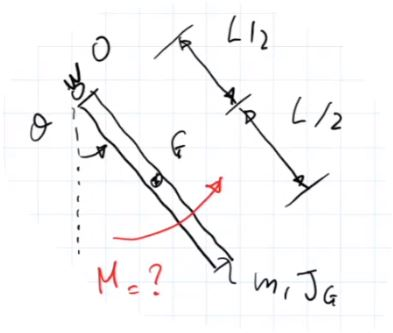
\includegraphics[height=3cm]{../lezione10/img3.JPG}
\end{center}
Sulla trave agisce un momento $M$ incognito e sono noti $\theta, \dot{\theta}, \ddot{\theta}$.\newline
Calcoliamo l'energia cinetica: $E_c = \frac{1}{2} m v_G^2 + \frac{1}{2} J_G \omega^2$, con $\omega = \dot{\theta}$ e $v_G = \dot{\theta} \frac{L}{2}$, per cui $E_c = \frac{1}{2} \left( m \frac{L}{4}^2 + J_G \right) \dot{\theta}^2$.\newline
Il teorema dell'energia cinetica ci dice che $W = \frac{dE_c}{dt}$, per cui ci basta calcolare la derivata dell'energia cinetica rispetto al tempo, ma ricordando che $E_c = E_c(\dot{\theta})$ possiamo sfruttare la derivata di funzione di funzione e ottenere quindi:
\[
    \frac{dE_c}{dt} = \frac{dE_c}{d \dot{\theta}} \frac{d \dot{\theta}}{ dt} = \left( m \frac{L}{4}^2 + J_G \right) \dot{\theta} \ddot{\theta}
\]
dove $\frac{d \dot{\theta}}{dt} = \ddot{\theta}$.\newline
A questo punto calcoliamo la potenza delle forze e coppie attive:
\[
    W = \vec{F}_P \; \text{x}\; \vec{v}_G + \vec{M} \; \text{x}\; \vec{\omega}
\]
con $\vec{F}_p$ forza peso.
\[
    W = mg \dot{\theta} \frac{L}{2} cos\left(\theta + \frac{\pi}{2}\right) + M \dot{\theta} = mg \dot{\theta} \frac{L}{2} (- sin(\theta))+ M \dot{\theta}
\]
Applicando ora il teorema dell'energia cinetica otteniamo l'equazione:
\[
    W = \frac{dE_c}{dt} \rightarrow -mg \frac{L}{2} \cancel{\dot{\theta}} sin(\theta) + M \cancel{\dot{\theta}} = \left( m \frac{L}{4}^2 + J_G \right) \cancel{\dot{\theta}} \ddot{\theta}
\]
\[
    M = \left(m \frac{L^2}{4} + J_G\right) \ddot{\theta} + mg \frac{L}{2} sin(\theta)
\]
\rule{\textwidth}{0,4pt}
\newpage
\section{Attrito}
L'attrito è la resistenza di impedimento al moto tra due corpi in contatto. L'attrito è sempre da considerarsi relativamente a due corpi in moto.\newline
\newline
\subsection{Modello di Coulomb}
Il modello di Coulomb per l'attrito tiene conto di tre evidenze sperimentali:
\begin{itemize}
    \item Per spostare un corpo in contatto con un altro bisogna applicare una forza, se non applico un certo livello di forza non riesco a instaurare un moto relativo fra i due corpi.
    \item La forza $\vec{F}$ che devo imporre per spostare un corpo lungo una superficia piana è tanto maggiore, tanto maggiore è il carico $P$ sul corpo che si vuole spostare.
    \item Se ho due corpi in movimento relativo uno rispetto all'altro, perchè questo movimento relativo permanga bisogna continuare ad applicare una forza o coppia, altrimenti il moto si arresta.
\end{itemize}
\ \newline
Distinguiamo due casi:
\begin{itemize}
    \item \textbf{Attrito statico}: se i corpi non sono in moto relativo.
    \item \textbf{Attrito dinamico}: se i corpi sono già in moto relativo fra loro. 
\end{itemize}
\subsection{Attrito statico}
Consideriamo due corpi a contatto.\newline
[immagine dagli appunti del prof]
\begin{center}
    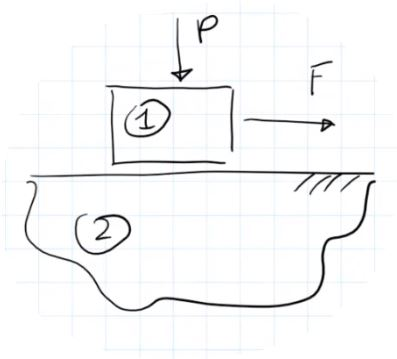
\includegraphics[height=3cm]{../lezione10/img4.JPG}
\end{center}
Per semplicità di trattazione consideriamo il corpo $2$ fermo (incastrato a terra), cioè con velocità nulla.